\chapter{Theory: semiconductor detectors}\label{chap:01}
In order to understand a silicone strip detector it is important to look at the theory of semiconductors.
%----------------------------------------------------%
\section{Electronic band structure}
Introduction to energy band theory in crystals.

X-ray analysis and other research have revealed that most metals and semiconductors possess a \emph{crystalline structure}, meaning an ordered atomic arrangement that repeats regularly in space. When forming this structure, the energy levels of electrons are altered. As atoms bond to form a crystal, the energy levels of the outermost shell electrons change most significantly since these electrons are shared between multiple atoms through covalent bonds.

The energy levels of these electrons can be determined through quantum mechanics. Specifically, electrons occupy not isolated single levels but \emph{bands} of allowed energies. The interval between a band's maximum and minimum energy is called the \enquote{band width}. Energy bands can be: valence bands, conduction bands, or forbidden bands.

The valence band is occupied by electrons shared between multiple atoms in the crystal, i.e., the band containing electrons farthest from the nucleus. The conduction band is the first empty band above it. Valence and conduction bands are separated by the \enquote{forbidden band}, an energy interval where no electrons can exist, whose width is typically denoted by \emph{Eg} (\enquote{energy band gap}).

As the distance between atoms in the crystalline structure decreases, the width of the forbidden band narrows until the conduction band overlaps with the valence band.  
The energy separation between valence and conduction bands determines whether materials are classified as insulators, semiconductors, or metals.

\begin{figure}[H]
       %\setkeys{Gin}{draft=false}
	\centering
	\fcolorbox{black}{white}{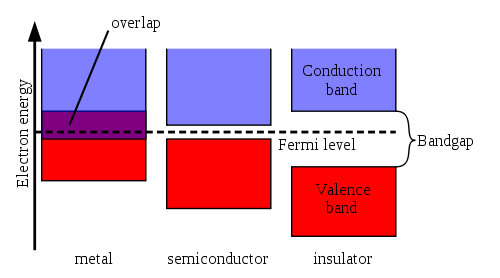
\includegraphics[scale=0.6]{pictures/conductionBand.png}}
	\caption{Energy band distribution in a metal, semiconductor, and insulator.}
	\label{fig:energyband}
\end{figure}

Insulators are materials where the forbidden band is wider than the energy an electron can acquire from an external field, preventing electrons from reaching the conduction band. Conversely, conductors have no forbidden band, with valence and conduction bands overlapping. This allows electrons to move freely to higher energy levels under an external field.

Finally, materials where valence and conduction bands neither overlap nor are separated by an impassable forbidden band (energetically) are called \emph{semiconductors}.
%----------------------------------------------------%
\section{Semiconductors}
In electronic components (e.g., diodes), the most common semiconductors are germanium [Ge] and silicon [Si]. At 0 K, these have Eg $\simeq$ 0.785 eV and Eg $\simeq$ 1.21 eV respectively – values exceeding the energy an electron typically gains from an external field to reach the conduction band. Thus, at this temperature, Ge and Si behave as insulators since no electron has sufficient energy to cross the band gap.  

As temperature increases, some electrons gain thermal energy > Eg and transition to the conduction band. These are called \emph{free electrons}, and the material becomes a \emph{semiconductor} due to its mobile charge carriers.  
Note that semiconductor conductivity increases with temperature, as higher temperatures generate more free electrons (charge carriers).

When an electron moves to the conduction band, it leaves an empty energy state in the valence band called a \emph{hole}.  
Thus, each electron in the conduction band corresponds to one hole in the valence band.  

\paragraph{def.} A \emph{intrinsic semiconductor} satisfies:
\[p=n\]
where p is hole concentration (valence band) and n is electron concentration (conduction band).  

If $p\neq n$, it is an \emph{extrinsic or doped semiconductor}.
%----------------------------------------------------%
\section{Doping of semiconductors}
Doping involves adding small percentages of trivalent or pentavalent impurity atoms to an intrinsic semiconductor to alter hole/electron density, creating an extrinsic semiconductor.  

(Ge and Si atoms are tetravalent)  
\begin{itemize}
	\item \textbf{Donors}: Pentavalent atoms added to the semiconductor (e.g., phosphorus [P]).  
	When bonding with lattice atoms, they form covalent bonds using four of their five valence electrons. The fifth electron remains mobile, becoming a charge carrier.  
	Donor doping is called \emph{n-type}, as it increases electrons and decreases holes (compared to intrinsic values).
	\item \textbf{Acceptors}: Trivalent atoms added to the semiconductor (e.g., boron [B]).  
	These form covalent bonds with only three of the semiconductor's four valence electrons, leaving a hole in the fourth bond.  
	Acceptor doping is called \emph{p-type}.
\end{itemize}

The semiconductor material utilized in this investigation is silicon, characterized by a band gap energy of 1.107 eV at room temperature \cite{labguide}. Silicon atoms possess four valence electrons and crystallize in a diamond cubic lattice configuration. Within this structure, electron vacancies (holes) emerge when valence electrons are displaced through thermal excitation or external particle interactions. These vacancies exhibit quasi-particle behaviour with an effective positive charge.

When subjected to an external electric field, established via cathode/anode contacts, the formation of bound electron-hole pairs (excitonic states) is suppressed. Under such bias conditions, liberated electrons and holes become mobile charge carriers that migrate toward the respective anode and cathode.

The electrical properties of silicon can be deliberately engineered through doping, a controlled substitutional process wherein host lattice atoms are replaced with impurity atoms possessing different valence electron counts. This atomic substitution modifies the charge carrier concentrations and transport characteristics.
%----------------------------------------------------%
\subsection{n-type semiconductors}
When silicon is doped with pentavalent impurities (e.g., arsenic, possessing five valence electrons), four electrons participate in covalent bonding with adjacent silicon atoms. The fifth electron remains weakly bound to its parent atom, requiring minimal energy (typically < 0.05 eV) to enter the conduction band as a mobile charge carrier. This process generates excess negative charge carriers without creating corresponding vacancies in the valence band.

\subsection{p-type semiconductors}
Doping with trivalent elements (e.g., boron, having three valence electrons) creates electron deficiencies in the crystal lattice. Each impurity atom forms incomplete covalent bonds with neighbouring silicon atoms, resulting in localized positive charge regions. These sites readily accept valence electrons from adjacent atoms, effectively generating mobile positive charge carriers known as holes that propagate through the lattice.

\autoref{fig:doping} schematically illustrates both doping mechanisms and their distinct effects on charge carrier generation in crystalline silicon.

\begin{figure}[H]
       %\setkeys{Gin}{draft=false}
	\centering
	\fcolorbox{black}{white}{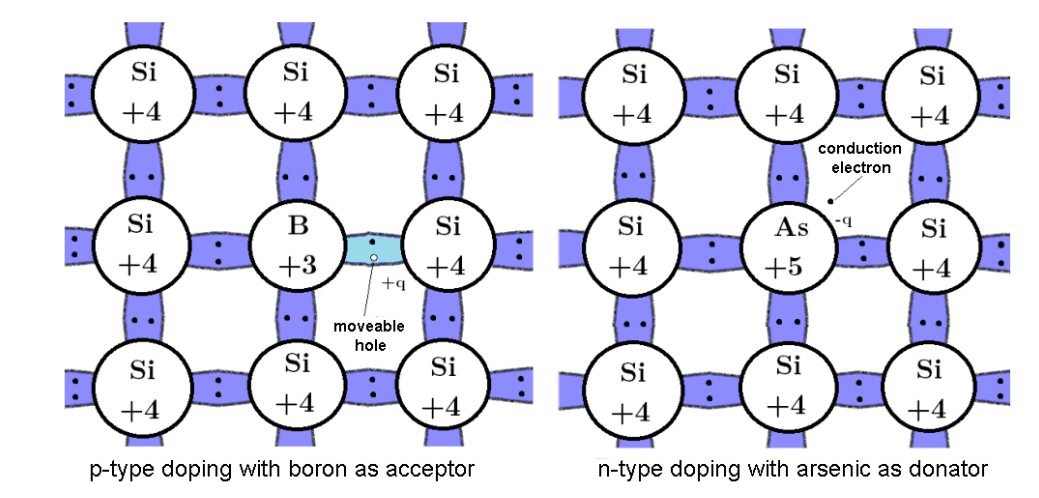
\includegraphics[scale=0.37]{pictures/doping.png}}
	\caption{Graphical representation of boron and arsenic doping in silicone.}
	\label{fig:doping}
\end{figure}
%----------------------------------------------------%
\section{The pn-junction}
The p-n junction is the contact region between p-type and n-type semiconductors, namely a \emph{diode}.  

Electrons (holes) approach the junction due to mutual attraction, leaving electrically neutral zones ($\rho=0$) at the far right (left) of the diode. The resulting central region is called the \endquote{depletion region}: a zone divided by the junction with thickness ~0.5 microns. Near the junction, high hole concentration in the p-region and low concentration in the n-region cause holes to diffuse from p to n, while electrons diffuse from n to p. This charge flow constitutes the diffusion current $I_{d}$ (direction: p to n). (Depletion width depends on doping and is inversely proportional to doping density on each side).  

Recombination starts at the junction and expands the depletion region until electron hole attraction can no longer overcome it. When the depletion width reaches equilibrium (where attraction is insufficient), recombination stops, leaving unrecombined \enquote{uncovered charges} on both sides.  
Thus, near the junction: the p-material has a region depleted of holes containing exposed negative charges, while the n-material has exposed positive charges.  

This creates:
\begin{itemize}
	\item $\rho=0$ at the junction due to recombination;
	\item $\rho>0$ on the n-side (peak at positive uncovered charges);
        \item $\rho<0$ on the p-side (minimum at negative uncovered charges). 
\end{itemize}  

This charge distribution generates an electric field (flux lines: positive → negative uncovered charges) and a \emph{diffusion voltage} $U_{D}$ opposing further diffusion. The depletion potential acts as a barrier that holes/electrons must overcome to diffuse into n/p-material respectively. Thus, $I_{d}$ depends on $V_{d}$, as the potential barrier height affects the number of free carriers and diffusion current.

To enable detection of ionizing radiation, an external bias voltage is applied across the diode terminals. Under reverse bias conditions:
\begin{itemize}
    \item Electrons from the negative terminal recombine with holes in the p-type region
    \item Electrons in the n-type region migrate toward the positive terminal
\end{itemize}
This charge carrier migration creates a charge-neutral region devoid of mobile carriers, known as the \textit{depletion zone}. The width $d(U)$ of this zone depends on the applied voltage $U$ according to:

\begin{equation}
    d(U) = \sqrt{ \frac{ 2 \epsilon (U_D + U) }{eN_{\mathrm{eff}} }}
\end{equation}
where: $\epsilon$ denotes the dielectric constant of silicon, $e$ is the elementary charge and $N_{\mathrm{eff}}$ represents the effective charge carrier density.

The effective charge carrier density is determined by the dopant densities in each region:
\begin{equation}
    N_{\mathrm{eff}} = \frac{ N_D N_A }{ N_D + N_A }
\end{equation}
with $N_D$ and $N_A$ being the donor (n-type) and acceptor (p-type) densities, respectively.

When the depletion zone spans the entire diode thickness $D$, full depletion occurs at the characteristic \textit{depletion voltage} $U_{\mathrm{dep}}$. This threshold voltage is approximated by:
\begin{equation}
    U_{\mathrm{dep}} \approx \frac{e N_{\mathrm{eff}} D^2}{2\epsilon}
\end{equation}

The depletion depth $d_c(U)$ exhibits distinct behaviour in two voltage regimes, characterized by the relationship:
\begin{equation}
d_c(U) = 
\begin{cases} 
D \sqrt{\dfrac{U}{U_{\mathrm{dep}}}} & \text{for}\hspace{5pt} U < U_{\mathrm{dep}} \\
\\
D & \text{for}\hspace{5pt} U \geq U_{\mathrm{dep}}
\end{cases}
\end{equation}

This functional dependence demonstrates that below the depletion voltage ($U < U_{\mathrm{dep}}$), the active detection region expands proportionally to the square root of the applied voltage. Once $U$ reaches or exceeds $U_{\mathrm{dep}}$, the depletion zone spans the entire diode thickness, saturating at $d_c = D$. This transition marks the optimal operating condition for radiation detection.

\begin{figure}[H]
       %\setkeys{Gin}{draft=false}
	\centering
	\fcolorbox{black}{white}{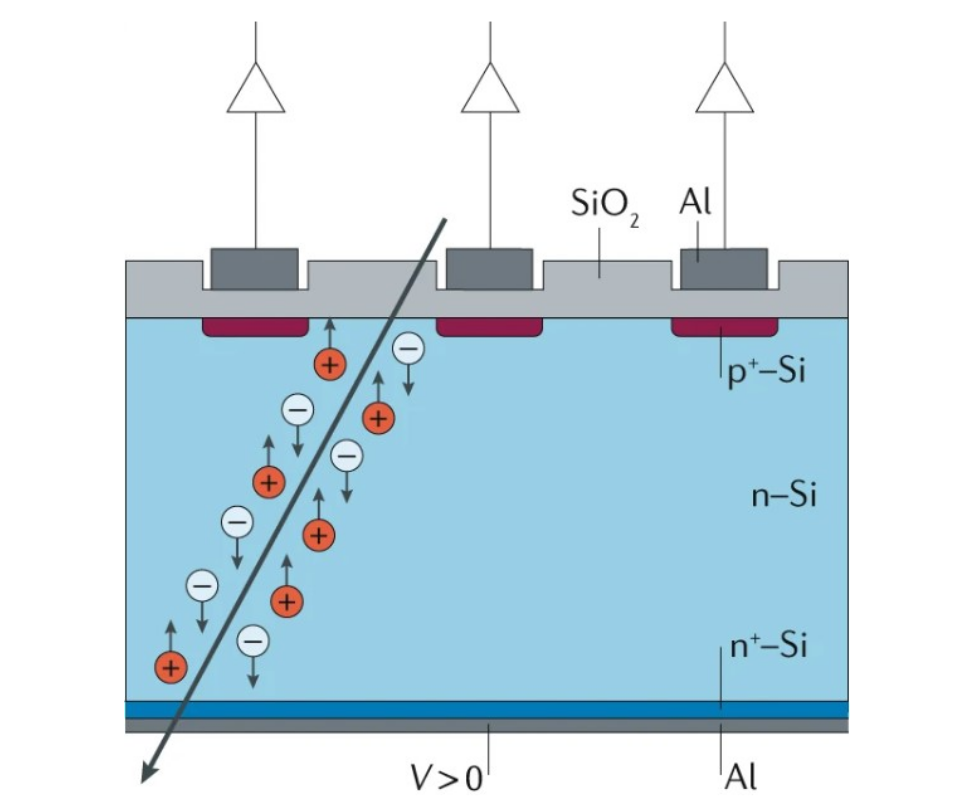
\includegraphics[scale=0.3]{pictures/ionizza.png}}
	\caption{Silicon strip detector crossed by a charged particle, from \cite{allport}.}
	\label{fig:ionization}
\end{figure}
%----------------------------------------------------%
\section{Interaction of ionising radiation with matter}

For effective detection of ionizing radiation, the diode should ideally operate in a fully depleted state. This condition maximizes the active detection volume, ensuring particle-induced charge carriers generate measurable signals. However, thermal excitation processes can promote electrons into the conduction band even without radiation, producing a \textit{leakage current}. 

The magnitude of this leakage current exhibits strong voltage dependence, increasing monotonically with applied bias. The characteristic current-voltage relationship for the detector diode is presented in Figure 2, which illustrates the transition between partial and full depletion regimes.

The depletion voltage ($U_{\mathrm{dep}}$), marking the onset of full depletion, can be determined through analysis of the current-voltage characteristics shown in \autoref{fig:currvolt}. This critical operational parameter corresponds to the voltage where the depletion region spans the entire diode thickness.

\begin{figure}[H]
       %\setkeys{Gin}{draft=false}
	\centering
	\fcolorbox{black}{white}{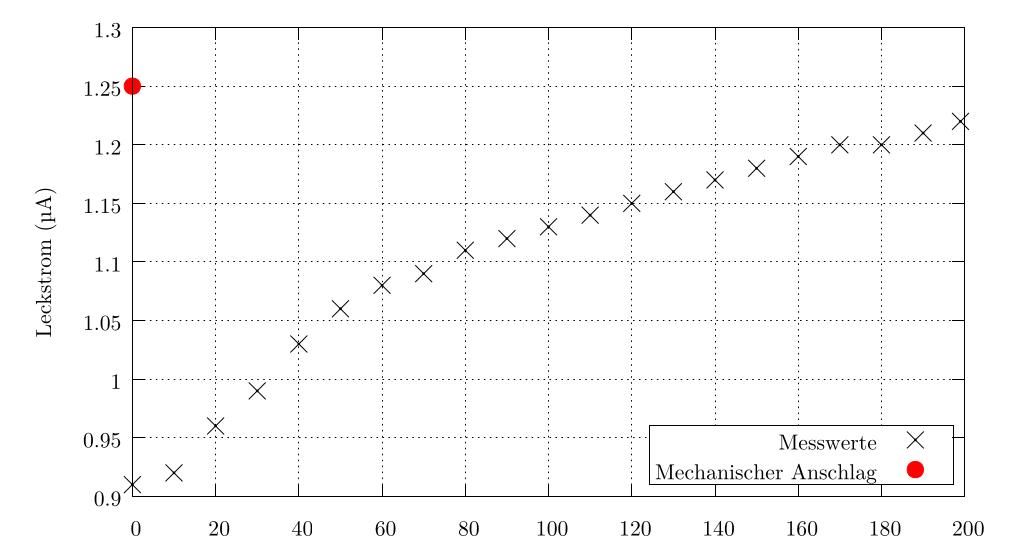
\includegraphics[scale=0.3]{pictures/currvolt.png}}
	\caption{Current-voltage characteristic curve of the Educational Alibava system. The depletion voltage $U_{\mathrm{dep}}$ can be estimated from the flattening of the curve at 60 V. Note that the adjustment knob for the bias voltage is not turned to the mechanical stop, as here the voltage is applied minimally in the forward direction, which leads to the value marked in red.}
	\label{fig:currvolt}
\end{figure}

The silicone strip detector can be used to detect ionizing particles. During the experiment a source producing beta particles is employed.

\subsection{The beta decay}

The primary radiation source utilized in this experiment is the $^{90}\mathrm{Sr}$ isotope, which undergoes $\beta^{-}$ decay according to the following sequence:

\begin{equation}
    {^{90}\mathrm{Sr}} \xrightarrow{\beta^{-}} {^{90}\mathrm{Y}} \xrightarrow{\beta^{-}} {^{90}\mathrm{Zr}}
\end{equation}

This decay chain produces two distinct $\beta^{-}$ emissions:
\begin{itemize}
    \item $^{90}\mathrm{Sr}$ $\rightarrow$ $^{90}\mathrm{Y}$ transition: $E_{\beta,\text{max}} = 0.545$ MeV
    \item $^{90}\mathrm{Y}$ $\rightarrow$ $^{90}\mathrm{Zr}$ transition: $E_{\beta,\text{max}} = 2.28$ MeV
\end{itemize}

During $\beta^{-}$ decay, a nuclear neutron transforms into a proton through the weak interaction process:

\begin{equation}
    n \rightarrow p + e^{-} + \bar{\nu}_e
\end{equation}

This three-body decay mechanism results in a continuous energy distribution for the emitted electrons, as the available Q-value is partitioned variably among the electron, antineutrino, and recoil nucleus. The characteristic energy spectrum for $\beta^{-}$ decay electrons is shown in \autoref{fig:betaDecay}.

\begin{figure}[H]
       %\setkeys{Gin}{draft=false}
	\centering
	\fcolorbox{black}{white}{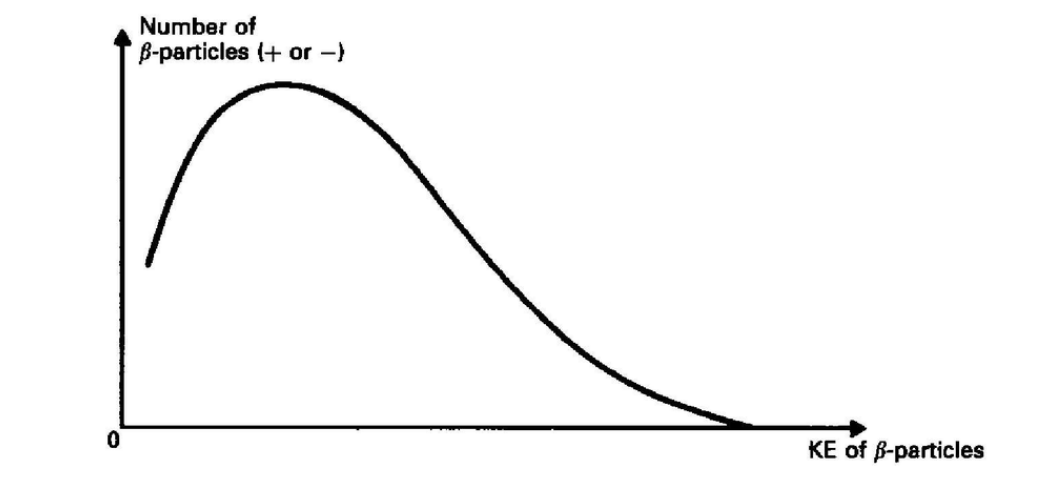
\includegraphics[scale=0.3]{pictures/betaDecay.png}}
	\caption{Electron energy spectrum of a $\beta^{-}$ decay, from \cite{corona}.}
	\label{fig:betaDecay}
\end{figure}

The temporal decay behaviour is quantified by the \textit{activity} $A$, defined as the disintegration rate:

\begin{equation}
    A \equiv -\frac{dN}{dt} = \lambda N_0 e^{-\lambda t} = A_0 e^{-\lambda t}
\end{equation}

where $\lambda$ denotes the decay constant, $N_0$ the initial number of radioactive nuclei, and $A_0$ the initial activity.

\subsection{interactions of electrons in matter}

Low-energy electrons ($E < 3$ MeV) predominantly lose energy through Coulomb interactions with atomic nuclei within the detector material. These ionizing collisions excite bound electrons in the semiconductor's crystalline lattice, producing electron-hole pairs that generate measurable detection signals. The average energy deposition per unit path length for relativistic electrons is described by the modified Bethe-Bloch formula:

\begin{equation}
    -\frac{dE}{dx} = 2\pi N_a m_e c \rho \frac{Z}{A} \frac{1}{\beta^2} \left[ \ln \left( \frac{\tau^{2}(\tau + 2)}{2(I/m_e c^2)^2} \right) + F(\tau) - \delta - 2\frac{C}{Z} \right]
\end{equation}
with the auxiliary function:
\begin{equation}
    F(\tau) = 1 - \beta^2 + \frac{\frac{\tau^2}{8} -(2r_e + 1)\ln(2)}{(\tau + 1)^2}
\end{equation}
where $\tau = \gamma - 1$; $\gamma$ is the Lorentz factor, and other parameters follow standard particle physics notation.

For electrons originating from the $^{90}\mathrm{Sr}$ decay spectrum, this formulation yields an average energy loss of 3.88 MeV/cm in silicon.

The statistical distribution of energy deposition events differs significantly with detector thickness. While bulk detectors ($\gtrsim$ 1 mm) exhibit approximately Gaussian energy loss distributions, thinner devices (such as the 300 $\mu$m detector employed here) demonstrate substantial deviations from normal statistics. In such thin absorbers, the energy loss distribution follows a Landau distribution, characterized by asymmetric broadening and a pronounced high-energy tail.

This distribution is further modified by the inherent energy spectrum of $\beta$-decay electrons, resulting in a convolution of the Landau distribution with the continuous $\beta$ energy spectrum. The composite energy deposition profile for our experimental configuration is presented in \autoref{fig:landau}.

\begin{figure}[H]
       %\setkeys{Gin}{draft=false}
	\centering
	\fcolorbox{black}{white}{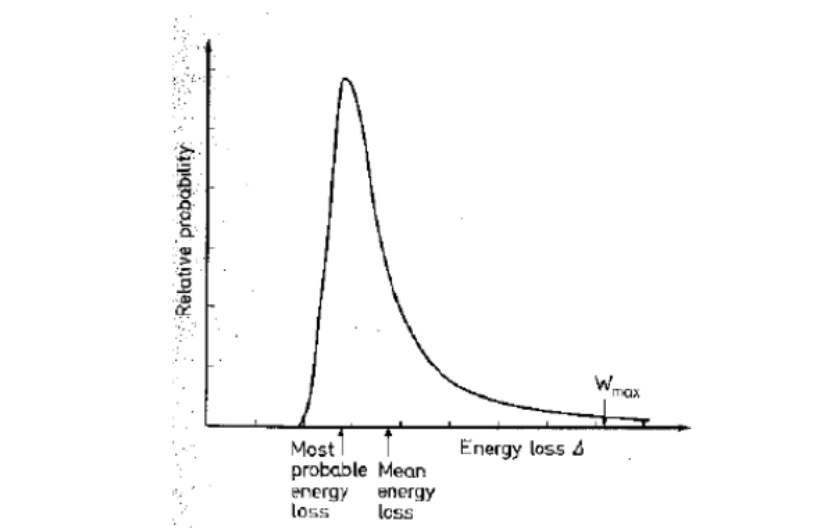
\includegraphics[scale=0.3]{pictures/landau.png}}
	\caption{Convoluted Landau distribution, describing the energy deposition of electrons in a 300 µm silicon sensor.}
	\label{fig:landau}
\end{figure}
%----------------------------------------------------%
\section{Pedestals and Noise}

All electronic measurement systems, including radiation detectors, exhibit inherent noise that obscures the desired signal. In this experiment, the charge deposition is given in counts of the Analog-to-Digital Converter (ADC) and therefore has to be converted to keV on the basis of a calibration measurement. For strip detectors interfaced with an ADC, the digitized output for strip $i$ during measurement $k$ follows:

\begin{equation}
\text{ADC}(i,k) = P(i) + D(k) + S(i,k)
\end{equation}
where:
\begin{itemize}
    \item $S(i,k)$ represents the true physical signal;
    \item $P(i)$ denotes the \textit{pedestal} (baseline offset) for strip $i$;
    \item $D(k)$ signifies the \textit{common mode shift} affecting all strips during measurement $k$.
\end{itemize}

The pedestal $P(i)$ is determined as the mean ADC response in the absence of physical signals:
\begin{equation}
P(i) = \frac{1}{N} \sum_{k=1}^{N} \text{ADC}(i,k) \label{eq:pedestal}
\end{equation}
where $N$ represents the number of noise measurements.

The common mode shift $D(k)$ quantifies system-wide electronic fluctuations and is computed via:
\begin{equation}
D(k) = \frac{1}{128} \sum_{i=1}^{128} \left[ \text{ADC}(i,k) - P(i) \right] \label{eq:shift}
\end{equation}

The intrinsic electronic noise per strip is characterized by the RMS deviation:
\begin{equation}
\sigma(i) = \sqrt{ \frac{1}{N-1} \sum_{k=1}^{N} \left[ \text{ADC}(i,k) - P(i) - D(k) \right]^2 } \label{eq:noise}
\end{equation}
This noise parameter $\sigma(i)$ provides the fundamental resolution limit for detecting physical signals on strip $i$.
%----------------------------------------------------%
